
\begin{figure}[H]
    \centering
    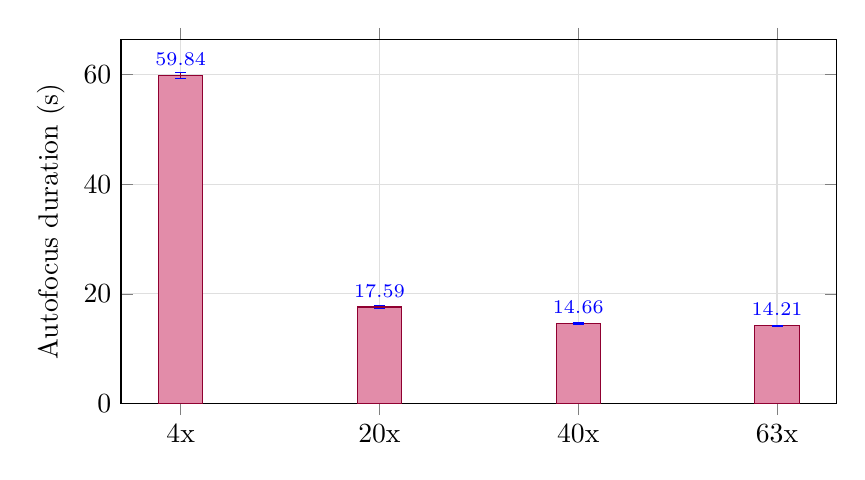
\begin{tikzpicture}
        \begin{axis}[
            width=0.88\linewidth,
            height=6.2cm,
            ybar,
            bar width=16pt,
            ymin=0,
            ylabel={Autofocus duration (s)},
            symbolic x coords={4x,20x,40x,63x},
            xtick=data,
            nodes near coords,
            nodes near coords align={vertical},
            every node near coord/.append style={font=\scriptsize},
            error bars/y dir=both, error bars/y explicit,
            grid=major,
            major grid style={draw=gray!25},
        ]
        \addplot+[fill=purple!45, draw=purple!75!black] coordinates {
(4x,59.8396) +- (0,0.4918)
(20x,17.5947) +- (0,0.3055)
(40x,14.6570) +- (0,0.1707)
(63x,14.2092) +- (0,0.0742)
        };
        \end{axis}
    \end{tikzpicture}
    \caption[Autofocus duration by objective]{Autofocus duration across objectives in the workflow-reliability evaluation. Each objective was run ten times successfully. Error bars show standard deviation. Focus stacking and tile scanning also completed 10/10 runs for each objective, but their durations were not recorded by the evaluation.}
    \label{fig:eval-workflow}
\end{figure}
